\documentclass{article}

\usepackage[brazil]{babel}

\usepackage{amsmath, amssymb}
\usepackage{graphicx}
\usepackage[colorlinks=true, allcolors=blue]{hyperref}

\usepackage{listings}
\lstset{
basicstyle=\small\ttfamily,
columns=flexible,
breaklines=true
}

\usepackage[section]{placeins}

\usepackage{tcolorbox}

\title{Relatório 03}
\author{Vinícius de Oliveira Peixoto Rodrigues (245294)}
\date{Março de 2023}

\begin{document}
\maketitle

\section{Introdução}

A tecnologia Wi-Fi é uma família de protocolos de rede sem fio, baseadas
na série de padrões IEEE 802.11, que definem as especificações para implementação
de tecnologias de rede wireless. As redes wireless são amplamente utilizadas para
construir redes de pequeno porte em aplicações domésticas ou de negócios.

A ferramenta \texttt{mininet} fornece um conjunto de ferramentas (disponibilizadas
como uma interface de linha de comando ou como uma interface em Python) que permite
a construção de arquiteturas de rede simuladas de forma rápida e fácil. Um fork dessa
ferramenta, chamado \texttt{mininet-wifi}, extende as funcionalidades da ferramenta
original, implementando suporte para simulação de redes Wi-Fi. Este experimento
busca explorar as funcionalidades da ferramenta \texttt{mininet-wifi}.

\section{Objetivos}

Este experimento básico tem como objetivo os seguintes pontos:

\begin{itemize}
    \item Explorar as funcionalidades da ferramenta \texttt{mininet-wifi}
    \item Compreender os princípios básicos de funcionamento de arquiteturas
          de rede wireless
    \item Fazer uso do simulador para investigar a relação entre parâmetros
          físicos e a performance de redes sem fio
\end{itemize}

\section{Metodologia}

O experimento dividiu-se em sete etapas:

\subsection{Primeiros passos}

Foi realizada a criação de uma topologia wireless básica, com um AP e duas estações
(\texttt{sta1} e \texttt{sta2}).
Em seguida, foram realizados testes básicos de conexão e desconexão entre as estações
e o access point; finalmente, foram realizadas medições de largura de banda entre as
duas estações.

\subsection{Exploração dos parâmetros do simulador}
Foi explorado o ajuste de parâmetros das estações no simulador, em particular o de
posição das estações. Além disso, foi realizada uma análise dos diversos parâmetros
de configuração disponíveis no simulador.


\subsection{Visualização da topologia wireless}




\subsection{Análise de quadros}
Análise de quadros 802.11 gerados pelo simulador no Wireshark


\section{Resultados e Discussão}

\subsection*{Parte 1}

\begin{tcolorbox}
    Qual é o atraso observado entre \texttt{sta1} e \texttt{sta2}?
    Houve perda de pacotes no canal? Justifique suas respostas de forma objetiva.
\end{tcolorbox}

\begin{figure}[!htb]
\centering
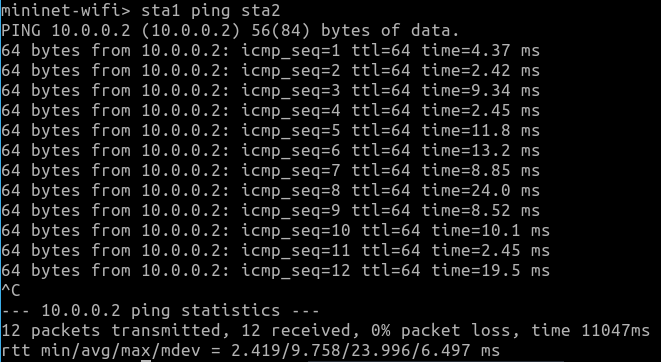
\includegraphics[width=\columnwidth]{images/p1_ping.png}
\caption{\texttt{ping} entre \texttt{sta1} e \texttt{sta2}.}
\end{figure}

O atraso médio observado na saída do comando \texttt{ping} é de 9.8 segundos.
Além disso, não foram observadas perdas de pacote.

\begin{tcolorbox}
    Use a ferramenta iperf para avaliar a banda disponível (Mbps)
    entre sta1 e sta2.
\end{tcolorbox}

\begin{figure}[!htb]
\centering
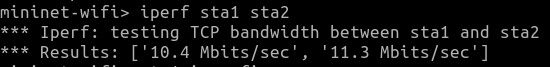
\includegraphics[width=\columnwidth]{images/p1_iperf.png}
\caption{Teste de largura de banda entre \texttt{sta1} e \texttt{sta2}.}
\end{figure}

\begin{figure}[!htb]
\centering
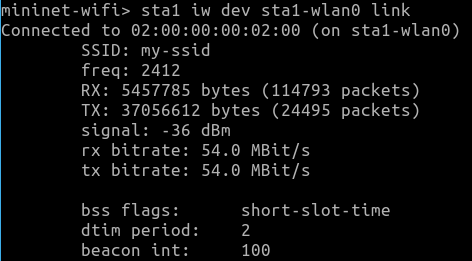
\includegraphics[width=\columnwidth]{images/p1_iwconfig.png}
\caption{Status do link \texttt{wlan} da estação \texttt{sta1}.}
\end{figure}

A largura de banda média entre as duas estações é de aproximadamente 11 Mbits/sec.
É interessante observar que a largura de banda na prática é significativamente menor que o
bitrate máximo negociado para os links \texttt{wlan} de cada estação.


\subsection*{Parte 2}

\begin{tcolorbox}
    Identifique a posição dos nós \texttt{sta1} e \texttt{sta2}.
\end{tcolorbox}

\begin{figure}[!htb]
\centering
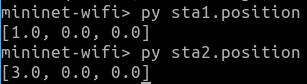
\includegraphics[width=\columnwidth]{images/p2_position.png}
\caption{Posição das estações \texttt{sta1} e \texttt{sta2}.}
\end{figure}

\FloatBarrier

\begin{tcolorbox}
    Investigue a lista de parâmetros de \texttt{sta1} (\texttt{py sta1.params}).
    Explique resumidamente qual informação do nó \texttt{sta1} cada item da lista representa.
\end{tcolorbox}

\begin{figure}[!htb]
\centering
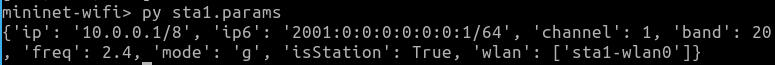
\includegraphics[width=\columnwidth]{images/p2_params.png}
\caption{Parâmetros de \texttt{sta1}.}
\end{figure}

Os parâmetros encontrados são:

\begin{itemize}
    \item \texttt{ip}/\texttt{ip6}: o endereço IPv4/Ipv6 atribuído à interface \texttt{wlan}
          da estação
    \item \texttt{channel}: o canal (isto é, faixa de frequências de operação) de
          acordo com a especificação 802.11g
    \item \texttt{band}: a banda (2.4 GHz) de comunicação wireless
    \item \texttt{freq}: a frequência da comunicação wireless
    \item \texttt{mode}: qual versão específica do protocolo 802.11 (neste caso,
          802.11g) na qual o canal está operando
    \item \texttt{isStation}: variável para identificação de estações Wi-Fi
    \item \texttt{wlan}: indica qual interface de rede (\texttt{sta1-wlan0}) está
          sendo usada para a conexão Wi-Fi


\end{itemize}

\end{document}
